\section{Introduction}

Dialogue system is an important interface between the machine and the human.  An intelligent dialogue agent is not only required to give the appropriate response based on the current utterance from the user, but also consider the dialogue history. Dialogue context modeling has been a key point for developing such dialogue systems, including researches on state tracking~\cite{abs-1907-01669,RenNM19}, topic segmentation~\cite{NanDNX19,kim2019dynamic}, multi-turn response selection~\cite{TaoWXHZY19,GuLL19}, next utterance generation~\cite{abs-1911-00536,ChenCQYW19}, etc. In this paper, we target on the multi-turn response selection task, which is first proposed by Lowe et al.~\shortcite{LowePSP15} and is also a track in both DSTC7~\cite{gunasekara2019dstc7} and DSTC8~\footnote{\url{https://github.com/dstc8-track2/NOESIS-II/}}.

%dialogue discourse parsing~\cite{BadeneTLA19,ShiH19},
%@inproceedings{BadeneTLA19,
%	author    = {Sonia Badene and
%		Kate Thompson and
%		Jean{-}Pierre Lorr{\'{e}} and
%		Nicholas Asher},
%	title     = {Data Programming for Learning Discourse Structure},
%	booktitle = {ACL},
%	pages     = {640--645},
%	year = {2019}
%}


%Dialogue context modeling has been a key point for developing such dialogue systems, including researches on state tracking~\cite{abs-1907-01669,RenNM19,RastogiGCM19}, topic segmentation~\cite{NanDNX19,kim2019dynamic,TakanobuHZLCZN18}, dialogue discourse parsing~\cite{BadeneTLA19,ShiH19,PerretAAM16}, multi-turn response selection~\cite{TaoWXHZY19,GuLL19,abs-1901-02609}, next utterance generation~\cite{abs-1911-00536,ChenCQYW19,LiuHLZ19}, etc.

%@inproceedings{RastogiGCM19,
%	author    = {Pushpendre Rastogi and
%		Arpit Gupta and
%		Tongfei Chen and
%		Lambert Mathias},
%	title     = {Scaling Multi-Domain Dialogue State Tracking via Query Reformulation},
%	booktitle = {NAACL-HLT},
%	pages     = {97--105},
%	year = {2019}
%}
%@inproceedings{TakanobuHZLCZN18,
%	author    = {Ryuichi Takanobu and
%		Minlie Huang and
%		Zhongzhou Zhao and
%		Feng{-}Lin Li and
%		Haiqing Chen and
%		Xiaoyan Zhu and
%		Liqiang Nie},
%	title     = {A Weakly Supervised Method for Topic Segmentation and Labeling in
%		Goal-oriented Dialogues via Reinforcement Learning},
%	booktitle = {IJCAI},
%	pages     = {4403--4410},
%	year = {2018}
%}
%@inproceedings{LiuHLZ19,
%	author    = {Cao Liu and
%		Shizhu He and
%		Kang Liu and
%		Jun Zhao},
%	title     = {Vocabulary Pyramid Network: Multi-Pass Encoding and Decoding with
%		Multi-Level Vocabularies for Response Generation},
%	booktitle = {ACL},
%	pages     = {3774--3783},
%	year = {2019}
%}


Given a dialogue history making up of more than one utterance, the selection task is to choose the most possible next utterance from a set of candidate responses.  Previous work on this task can be roughly divided into two categories: sequential models and hierarchical models. The former ones, including \cite{LowePSP15,YanSW16,abs-1901-02609}, concatenate the history utterances into a long sequence, try to capture the similarities between this sequence and the response and give a matching score. The latter ones, including \cite{TaoWXHZY19,WangWC19,GuLL19}, extract similarities between each history utterance and the response first. Then, the matching information aggregated from each pair 
(mostly in a chronological way) to get a final score. 
There is little difference between the performance of these two kinds of 
architectures until the emergence of large pre-trained language models.
 
 \begin{figure}
 	\centering
 	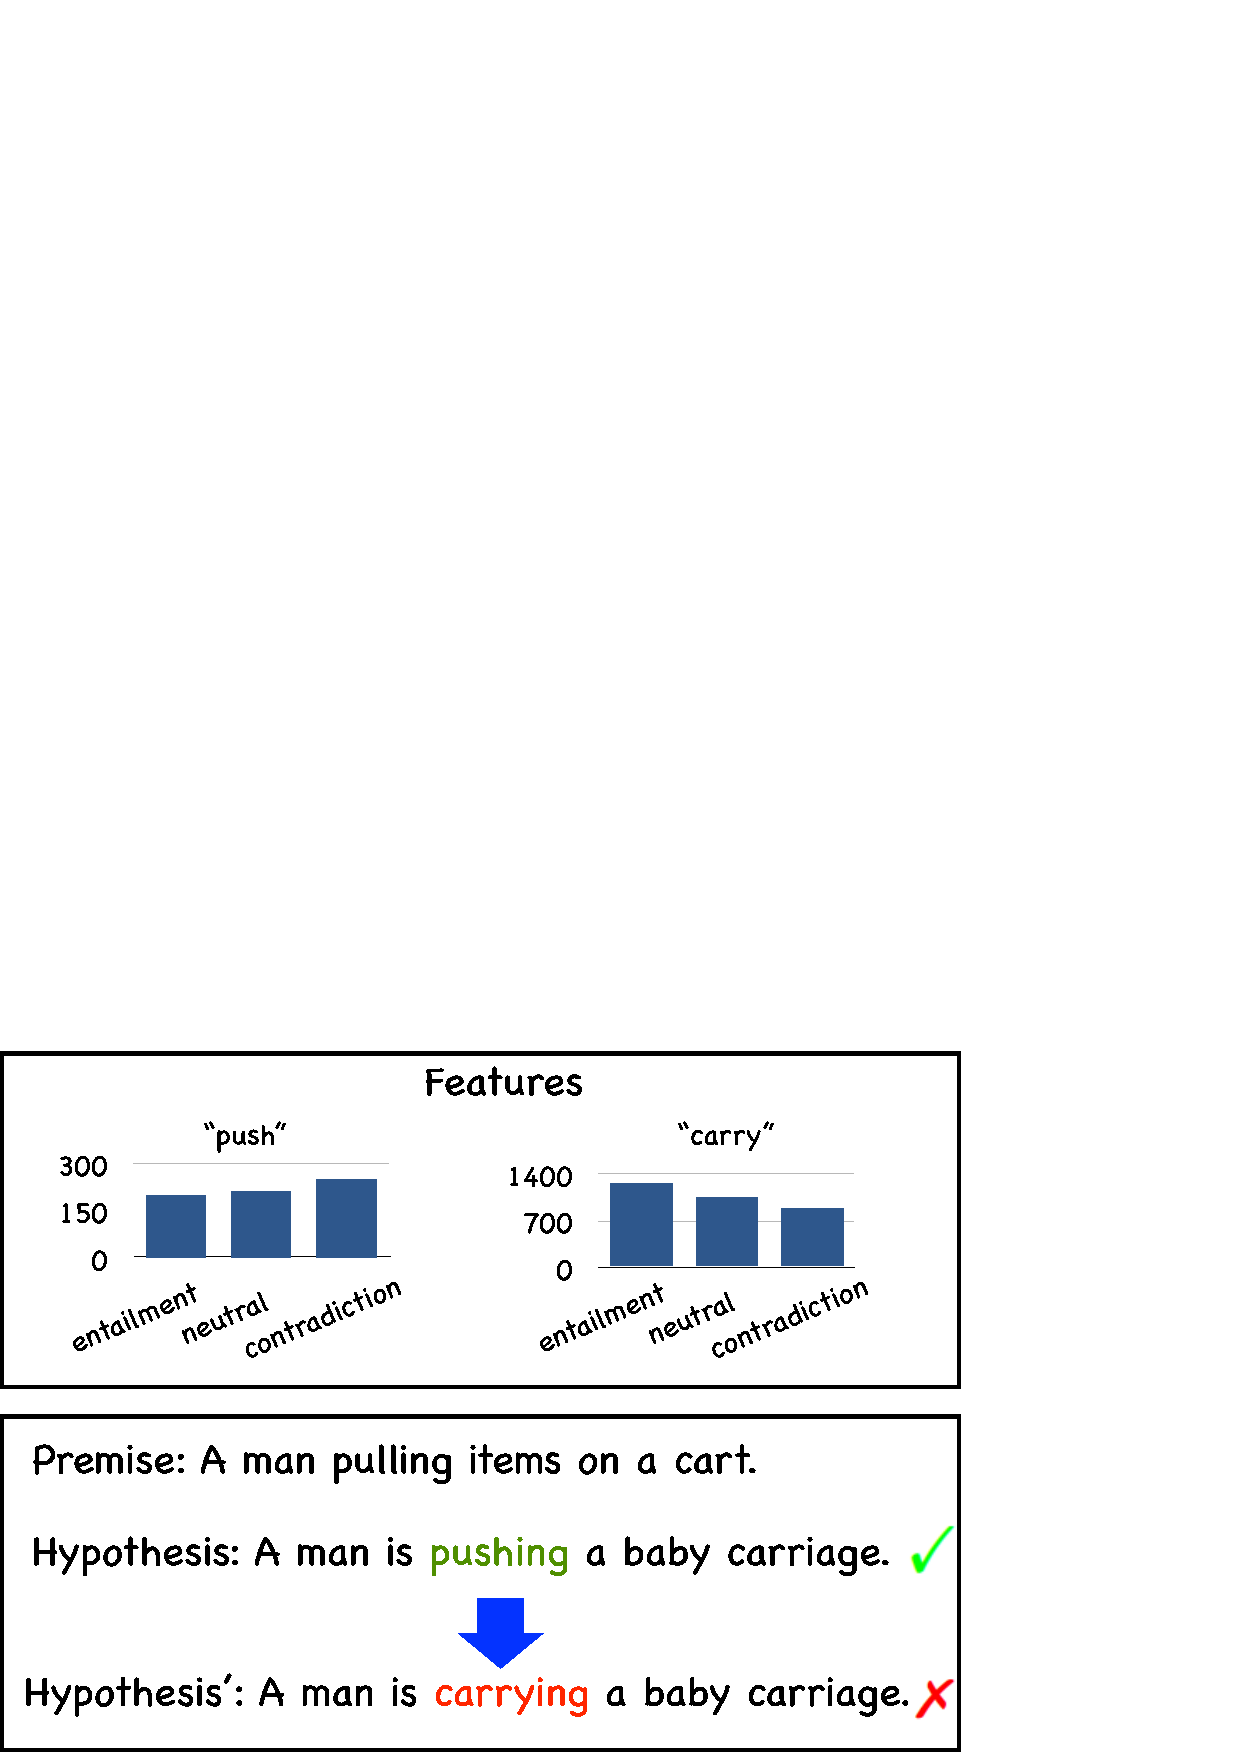
\includegraphics[scale=0.43]{pic/example.pdf}
 	\caption{An example of the tangled dialogue history. A, B and C are three participants. Texts in different colors represent different dialogue threads.}
 	\label{fig:example}
 \end{figure}
 
 
Work such as \cite{abs-1908-04812,vig2019comparison} has shown the 
extraordinary performance of the pre-trained language models on dialogues. 
These pre-trained models are easily transferred to the response selection 
task by concatenating all of the utterances as the input. 
All of the words in the dialogue history can directly interact with each other 
via transformers like Bi-encoder, even the words both in the dialogue history 
and response if time permits, such as Cross-encoder~\cite{humeau2019poly}. 
However, since such models can be regarded as the ultimate 
architecture of the sequential-based models, the dialogue dependency 
information between the utterances is largely ignored due to the 
concatenation operation~\cite{WuWXZL17}. An example is shown in Figure \ref{fig:example}. The dependency relations can definitely help us to understand the two tangled dialogue threads.
%\KZ{Why is the dependency information important? Here you can include an example.} 
Besides, we always need to truncate the earlier dialogue history 
to limit the size of the model and make the computation efficient, 
but it isn't always that the nearest utterances are more important. 
As we can see in Figure \ref{fig:example}, several dialogue threads may 
be tangled especially in multi-party chat rooms, 
it's hard to tell which dialogue thread will be moving on.
%\KZ{I think the second point is related to the first point.}

In this paper, we propose to incorporate dialogue dependency information 
into the response selection task. Previous work on discourse parsing for 
dialogues are based on the SDRT theory~\cite{0031949}. This theory takes 
a clause-level units as elementary discourse units (EDUs) and defines 16 relations types. Annotating dialogues under such theory requires domain experts and is time-consuming. We relax the definition of dependency relations in dialogues, 
by taking each utterance as the basic unit and focusing only on 
the ``reply-to'' relation type. In this way, labeling training data for 
predicting dependency relations by crowd-sourcing becomes possible and more
reliable.

%\KZ{The first, then, finally... seem to describe a process. But in
%this process you used words such as ``design'', ``propose''. This is 
%weird.}
Using the trained dialogue dependency parser, we parse the dialogue 
to find the most probable parent utterance for each utterance in the session. 
Then, we empirically design an algorithm to exact dialogue threads which is represented by a path of dependency relations.
%\KZ{we empirically design an algorithm to cut the dialogue history turns into several segments based on the predicted dependency relations.} 
%\KZ{I think we should use the word ``extract''. Extract dialogue threads
%which is represented by a path of dependency relations.}
%Each segment is considered as an individual dialogue thread, 
The extracted threads are sorted by the distance between the final utterance in each 
thread and the response in ascending order, following the intuition that the closer utterances are more relevant.
%\KZ{You should explain why we
%do sorting here.} 
Finally, we propose the model named Thread-Encoder, which is based on the pretrained language 
model. 
%\KZ{Not sure what you mean by ``block''. Maybe u should refer to the
%fig here.} 
The pretrained model 
distills the critical information from each dialogue thread. 
Another attention layer is used to calculate the final matching score 
with the thread representations and the candidate representation. 

We collect the training data for dependency parsing from a dialogue 
disentanglement dataset~\cite{KummerfeldGPAGG19} in a technical domain. 
Since the dialogue parser is trained in a technical domain,  
we do experiments among UbuntuV2, DSTC7 dataset and DSTC8 dataset. 
These datasets consist of dialogues in the same domain but under different settings, 
including two-party dialogues and multi-party dialogues. 
The results demonstrate our model's strong capability to represent multi-turn
dialogues on all these datasets.

 
Our main contributions are as follows:
\begin{itemize}
	\item As far as we know, we are the first to incorporate dialogue 
dependency information into response selection task, 
demonstrating that the dependency relations in the dialogue history 
are useful in predicting dialogue responses (Section \ref{sec:relatedwork}). 
	\item Based on the predicted dependencies, we design a straight-forward but effective algorithm to extract several threads from the dialogue history  (Section \ref{sec:DSA}). 
The results show the algorithm is better than other simple segmentation 
methods on the response selection task.
	\item We propose the Thread-Encoder model, incorporating dialogue 
dependency information by threads and utilizing the pre-trained language 
model to generate corresponding representations (Section \ref{sec:tem}). The experimental results 
show that our model outperforms the state-of-the-art baselines on 
both DSTC7 and DSTC8 datasets, and is very competitive on UbuntuV2 (Section \ref{sec:ra}).
\end{itemize}





